\chapter{Solido}

\section{Práctica 1: }
\section{Práctica 2: }
\section{Práctica 3: }
\section{Práctica 4: }
\section{Práctica 5: }
\section{Práctica 6: }
\section{Práctica 7: }
\section{Práctica 8: }



\newpage

\section*{\textit{Examenes resueltos}}
\addcontentsline{toc}{section}{\textit{Examenes resueltos}}

\subsection*{\textit{2024}}\begin{Enunciado}
	\addcontentsline{toc}{subsection}{\textit{2024}}

	\subsubsection{Difracción de rayos X (Elisa Casal)}
	Preguntas
	\begin{enumerate}[label=\alph*)]
		\item Se tiene una muestra policristalina en polvo de un material con estructura bcc de parámetro de red 4 Å. Si se realiza un difractograma de rayos X con una longitud de onda \( \lambda = 1.540\ \text{\AA} \), ¿a qué ángulos \( \theta \) aparecen los tres primeros picos de difracción?
		\item Si los ángulos de todos los picos de difracción estuviesen sobreestimados en aprox. \( 1^\circ \), ¿las constantes de red que se obtienen estarán sobreestimadas o subestimadas?
	\end{enumerate}
\end{Enunciado}


Solución
\begin{enumerate}[label=\alph*)]
	\item La ecuación que tenemos que usar es la siguiente:

	      \begin{equation}
		      \sin (\theta)=\frac{\lambda}{2a}\sqrt{h^2+k^2+l^2}
	      \end{equation}

	      No obstante, es necesario particularizarla según el criterio de selección de (h,k,l) para una FCC que es que h+k+l ha de ser par. Teniendo esto en cuenta para las tres primeras ternas que verifican el criterio de selección tenemos:

	      \begin{itemize}
		      \item (1,1,0) $\longrightarrow$ $\theta_1$=15.80º
		      \item (2,0,0) $\longrightarrow$ $\theta_2$=22.64º
		      \item (2,1,1) $\longrightarrow$ $\theta_3$=32.98º
	      \end{itemize}

	\item Si todos los ángulos medidos están sobreestimados tenemos $\theta_{\text{medida}}>\theta_{\text{real}}$. Para los ángulos de arriba ello implica: $\sin(\theta_{\text{medida}})<\sin(\theta_{\text{real}})$. Considerando que $a \propto 1/\sin(\theta)$ obtendríamos $a_{\text{medida}}<a_{\text{real}}$, es decir, obtenemos un valor infraestimado para la constante de red.
\end{enumerate}

\vspace*{2em}

\begin{Enunciado}
	\subsubsection{Fotoconductividad}
	Preguntas
	\begin{enumerate}[label=\alph*)]
		\item Confirma o refuta la siguiente afirmación: ``La conductividad de exceso, que se define como la conductividad por encima de la ambiental, resulta seguir una ley no lineal (en concreto, potencial) con la irradiancia recibida por el fotorreceptor, con un exponente ligeramente mayor que la unidad''.
		\item ¿Cómo mediste la conductancia intrínseca $G_0$? ¿Es mayor o menor que la que se obtiene con la luz de la bombilla incidiendo sobre la fotocélula?
	\end{enumerate}
\end{Enunciado}

Solución:

\begin{enumerate}[label=\alph*)]
	\item Aunque efectivamente la conductividad de exceso de define como la conductividad por encima de la ambiental, es decir:
	      \begin{equation*}
		      \Delta G (\Phi) = G(\Phi)  - G_0
	      \end{equation*}
	      siendo $\Phi$ la irradiancia, la relación no es lineal, es efectivamente potencial (con la raíz cuadrada), tal y como vamos a demostrar aquí. La realción con el número de portadores $n$ del exceso de conductividad es tal que
	      \begin{equation*}
		      \Delta G \propto n(\Phi) - n_0
	      \end{equation*}
	      y, el número de portadores $n(\Phi)$, a su vez, una relación no lineal con la irradiancia
	      \begin{equation*}
		      \gamma n(\Phi)^2 = \beta  \Phi
	      \end{equation*}
	      Es decir, la relación de la conductividad de exceso y la irradiancia se relaciónan a través de la raiz cuadrada:

	      \begin{equation*}
		      \Delta G \propto \sqrt{\Phi}
	      \end{equation*}
	      en general, al no tener una fuente monocromática, en realidad

	      \begin{equation*}
		      \Delta G \propto \Phi^{m/2}
	      \end{equation*}
	      siendo $m$ un valor que debería rondar sobre 1. Experimentalmente se obtuvo (Daniel Vázquez Lago) un valor $m\approx 1.06$, mientras que en otras prácticas (Raquel Alfonso) se obtuvo $m\approx 1.3-1.6$.

	\item La conductancia intrísneca que es la conductancia que tiene el el fotodiodo cuando está aislado (no recibe ningún tipo de irradiancia ambiental o externa). Para medirla estudiamos $I$ frente a $V$, tal que la ley de Ohm y una regresión lineal nos dará el valor de $G_0$:
	      \begin{equation*}
		      V = G_0 I
	      \end{equation*}
	      Es menor que la que se obtiene con la luz de la bombilla incidiendo sobre la fotocélula, ya que la luz genera un exceso de portadores al excitar electrones en la banda de valencia del semiconductor.
\end{enumerate}

\vspace*{2em}

\begin{Enunciado}
	\subsubsection{Conductividad eléctrica de placa dentada}
	Preguntas
	\begin{enumerate}[label=\alph*)]
		\item En la imposición de condiciones de contorno sobre la corriente de entrada, \textit{Agros2D} pide la densidad de corriente. ¿Cómo se obtiene la sección para determinar dicha densidad de corriente a partir de la intensidad?
		\item Indica y explica brevemente la regla de proporcionalidad que se aplica para la determinación de $\sigma$ a partir de los resultados de la simulación.
	\end{enumerate}
\end{Enunciado}

Solución:

\begin{enumerate}[label=\alph*)]
	\item La densidad de corriente de entrada $J$ y la intensidad que medimos en el laboratorio se relacionan de la siguiente manera:
	      \begin{equation*}
		      J = \frac{I}{A}
	      \end{equation*}
	      siendo este área el área que está alrededor del tornillo, véase

	      \begin{equation}
		      A = 2 \pi r \cdot d
	      \end{equation}
	      siendo $r$ el radio del borne y $d$ el espesor de la placa.
	      \begin{figure}[H] \centering
		      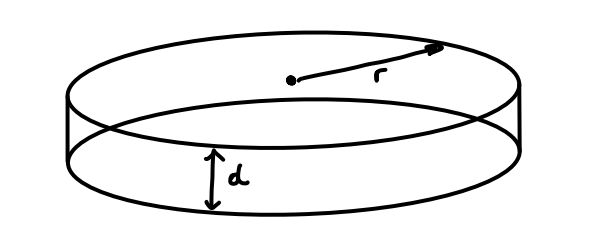
\includegraphics[width=0.6\linewidth]{Cuerpo/Ch_02/Examen_24_3.png}
	      \end{figure}
	\item La relación entre $\sigma_{\exp}$ y $\sigma_{sim}$ basicamente nos dice que:

	      \begin{equation*}
		      V_{\exp} \sigma_{\exp} = V_{sim} \cdot \sigma_{sim}
	      \end{equation*}
	      donde $\sigma$ es la conductividad y $\rho=1/\sigma$ sería la resistividad. El funcional de resistencia $R(\rho)$ depende de la resisitividad del metal y de la forma geométrica, que por definición dependerá linealmente de la resistividad $R(\rho) \propto \rho$ (piensa en las unidades, debe ser necesariemente lineal ya que $R$ va con $\Omega$ y $\rho$ va con $\Omega \cdot m$),y por tanto entre 2 metales con la misma forma:

	      \begin{equation}
		      \frac{R_{sim}}{R_{\exp}} = \frac{\rho_{sim}}{\rho_{\exp}}
	      \end{equation}
	      Y si ambos tienen la misma intensidad entonces la ley de Ohm (que en un metal se cumple siempre)

	      \begin{equation*}
		      V = R(\rho) I \longrightarrow I = \frac{V}{R(\rho)}
	      \end{equation*}
	      Finalmente, si $\rho = 1/\sigma$, efectivamente:

	      \begin{equation*}
		      V_{\exp} \sigma_{\exp} = V_{sim} \cdot \sigma_{sim}
	      \end{equation*}
	      \textbf{Resumen}: en el caso de que la geometría de dos objetos sea igual, ambos sean óhmicos y que les atraviese la misma corriente por los bordes, entonces la relacion voltaje x conductividad será igual en ambos.
\end{enumerate}

\vspace*{2em}
\begin{Enunciado}
    \subsubsection{Conductividad eléctrica de placa perforada (Elisa Casal)}
    Preguntas
    \begin{enumerate}[label=\alph*)]
    \item ¿A qué puntos se les impuso la condición de contorno de voltaje nulo? Discute brevemente por qué.
    \item En la simulación por elementos finitos, ¿de qué modo y dónde entraba el espesor de la placa metálica?
    \end{enumerate}
    \end{Enunciado}
    
Solución
\begin{enumerate}[label=\alph*)]
	\item El voltaje nulo se le puso como condición de contorno al terminal de salida.

	\item El espesor entra en juego para establecer la $J_0$ en la condición de contorno sobre el terminal de entrada.

	      Nosotros lo que hemos medido previamente a la simulación es $I_0$, que es la corriente que establecimos en las medidas experimentales y el $V_{exp}$ al que da lugar esta corriente. Como para introducir en el \textit{Agros2d} lo que necesitamos es una denisdad de corriente habrá que dividir $I_0$ entre el área tranversal que atraviesa. Este es un método que puede introducir mucha incertidumbre. El área tranversal que atraviesa la corriente será la longitud, \textit{L}, del terminal multiplicada por el espesor, \textit{d}, de la placa. Esa longitud, en principio, debería de ser la de los tres lados que forman el terminal. De esta manera la denidad de corriente para introducir como condición de contorno en el terminal de entrada es:

	      \begin{equation}
		      J_0=\frac{I_0}{L \cdot d}
	      \end{equation}
\end{enumerate}

\vspace*{2em}

\begin{Enunciado}
	\subsubsection{Temperatura de Debye}
	Preguntas
	\begin{enumerate}[label=\alph*)]
		\item Si tenemos en cuenta el intercambio de calor entre nuestro sistema (vaso con agua más muestra) con el ambiente durante el proceso de enfriamiento que experimenta el agua al introducir la muestra de cobre, ¿la temperatura final del agua es mayor o menor que la medida experimentalmente? ¿Y qué sucede con $\Theta_D$? ¿Aumenta o disminuye?
		\item Teniendo en cuenta el procedimiento experimental que seguimos en la práctica, ¿con qué tipo de material sería más “fácil” (en el sentido de precisa) la determinación de $\Theta_D$? ¿Con uno de $\Theta_D$ muy baja (digamos $\Theta_D \approx 50\ \text{K}$) o con otro de $\Theta_D$ muy alta (digamos $\Theta_D \approx 600\ \text{K}$)? ¿Y con respecto a la masa de la muestra? ¿Es mejor que sea más ligera o más pesada?
	\end{enumerate}
\end{Enunciado}

Solucion:

\begin{enumerate}[label=\alph*)]
	\item Si consideramos el intercambio de calor entre nuestro sistema (vaso con agua + muestra) y el ambiente, la temperatura final del agua \textit{medida experimentalmente será mayor que la real}. Esto ocurre porque, durante el proceso, el agua gana energía del ambiente al estar mas frío que este. Por tanto, la medida de $T_f$ será algo mayor que si el sistema estuviese perfectamente aislado, de tal modo que $\Delta T_{agua}$ es menor. consecuentemente, el valor $\Delta U_{\exp}$ será menor también que en el caso aislado.

	      Ahora, veamos que la siguiente gráfica en la que representamos $C_V$ frenet $T$ y $T/\theta_D$ respectivamente.

	      \begin{minipage}{0.47\linewidth}
		      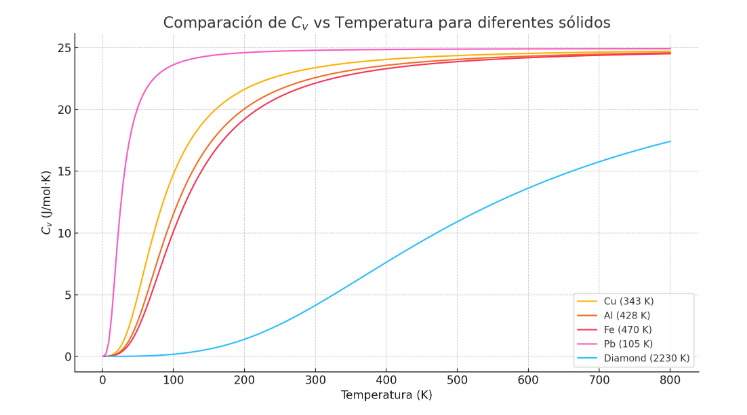
\includegraphics[width=1\linewidth]{Cuerpo/Ch_02/Examen_24_5-2.png}
	      \end{minipage} \hfill
	      \begin{minipage}{0.47\linewidth}
		      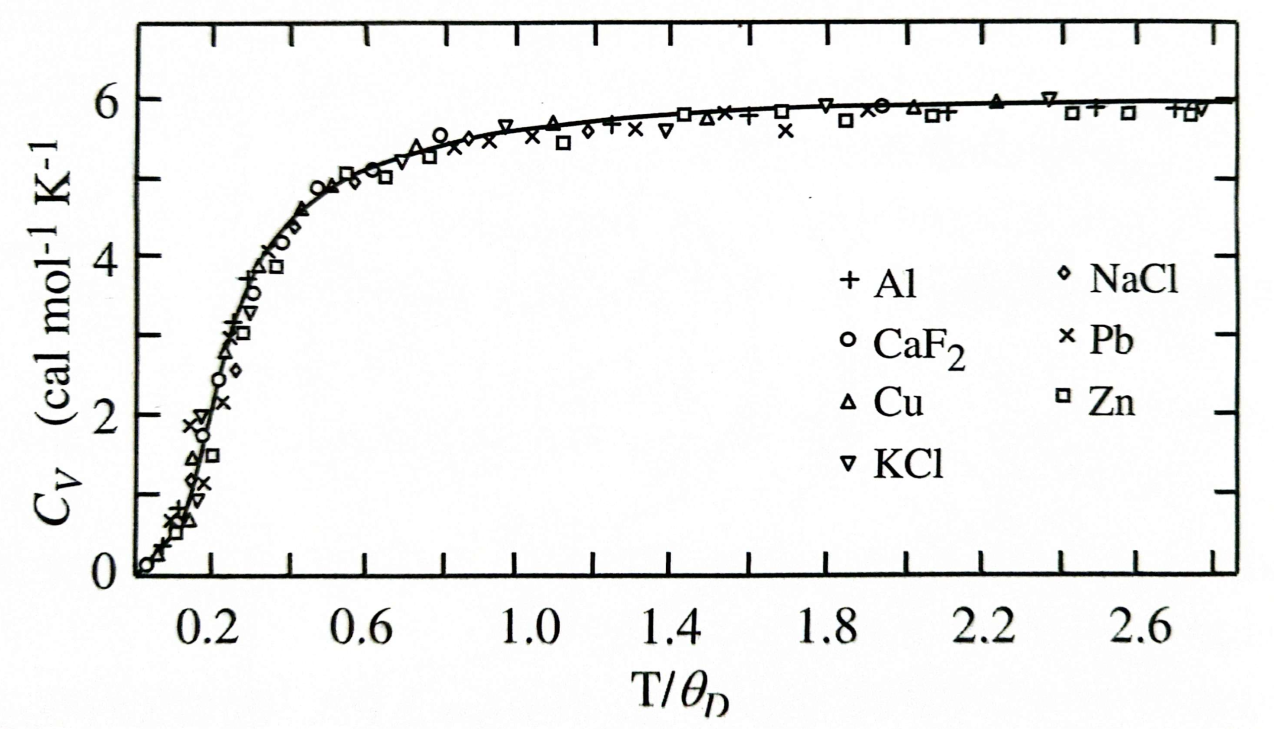
\includegraphics[width=1\linewidth]{Cuerpo/Ch_02/Examen_24_5-3.png}
	      \end{minipage}

	      Dado que $\Delta U$ entre entre dos valores de $T/\Theta_D$ es la integral debajo de la curva de $C_V$:

	      \[
		      \Delta U_{\text{teo}} = \int_{T_i}^{T_f} C_V(T)_{\text{cobre}} \D T
	      \]

	      Y por tanto tenemos que efectivamente cuando mas alto $T/\theta_D$ aumenta el valor de $\Delta U$. Si aumentamos $T_f \uparrow$ (recordamos que $T_i=73$ K es fijo, el valor del nitrógen líquido), tenemos que $\Delta U_{\text{teo}} \uparrow$, sin embargo tenemos experimentalmente que $\Delta U_{\exp} \downarrow$. Así pues, la única forma de obtener un $\Delta U_{\text{teo}} \downarrow$ cuando $T_f \uparrow$ es aumentar $\theta_D \uparrow$. Es decir, $\theta_D$ experimental aumentará respecto al valor aislado. De hecho es lo que ocurre experimentalmente, ya que $\theta_D=343$ K (cobre) y experimentalmente en el laboratorio de mide $\theta_D \approx 360$ K (Elisa Casal).

	\item Si tenemos un material $\theta_D\approx 600$ K estaremos en el límite cuántico ($T<\Theta_D$), mientras que $\theta_D \approx 50$ K estaremos en el límite clásico. Si le echamos un vistazo a a laimagen .

	Como podemos ver, en el límite clásico, una variación de temperatura pequeña puede alterar bastante el valor de la energía interna, mientras que en el límite cuántico necesitaremos mayor temperatura para obtener la misma $\Delta U$. Necesitar menos temperatura, o que con la misma diferencia de temperatura inicial y final pueden mejorar bastante los resultados: mas diferencia habrá entre la temperatura inicial y final del agua, y por tanto mayor sensibilidad. Hablamos de temperatura de la muestra. Es decir, \textit{preferimos una temperatura de Debye baja}.

	Sin embargo es posible que alguién quiera barajar la idea de que para $\Theta_D$ baja $C_V$ no depende realmente de $\Theta_D$, y por tanto variar $\Theta_D$ cuando calculamos el valor $\Delta U_{\exp}$ para que se verifique $\Delta U_{\exp}\approx \Delta U_{\text{teo}}$. El autor no es particularmente seguidor de esta idea, ya que aunque esto es verdad uno va a seguir usando las ecauciones de $D_3(T)$ igual (por lo que el error debido a usar la aproximación será "el mismo"), además de ser una explicación bastante más compleja y que habría que ver si realmente sucede numéricamente. En cualquier caso habría que considerarla como un argumento en contra de $\Theta_D$ baja. Si a alguien se le ocurre otra idea que contacte conmigo.


	Respecto a la masa de la muestra, una muestra más pesada intercambia más calor con el agua (mayor $\Delta U$), ya que es capaz de ``almacenar más energía en su interior''. Es decir, para el mismo material cobre, más masa implica más moles, y más moles de cobre implican que $\Delta U$ será mas grande para el mismo $\Delta T$, y por tanto mayor sensibilidad.
\end{enumerate}

\vspace*{2em}

\begin{Enunciado}
	\subsubsection{Efecto Hall en semiconductores}
	Preguntas
	\begin{enumerate}[label=\alph*)]
		\item Supón que, debido por ejemplo a un efecto termoeléctrico, en toda la experiencia las lecturas de caída de voltaje entre los terminales transversales del semiconductor tienen una contribución extra de \(-0.1\,\text{V}\), y que no la corregimos. ¿Cómo afectaría ello al valor obtenido para el coeficiente Hall \( R_H \)?
		\item En un montaje experimental dado, con polaridades fijas de las conexiones entre la muestra, fuentes y demás equipamiento, cuando se consideran casos de conductores por electrones o por huecos, ¿las fuerzas de Lorentz tienen igual signo o signos opuestos en un caso frente al otro?
	\end{enumerate}
\end{Enunciado}

\begin{enumerate}[label=\alph*)]
	\item No, no nos afecta, ya que lo que nosotros usamos para calcular el efectp Hall es usar la pendiente de la curva, la cual no se ve afectada al aumentar $I$ uniformemente. Aumentar $I$ uniformemente solo modifica el término independiente.

	\item Las fuerzas de Lorentz actúan en el mismo sentido. Ingénuamente uno podría pensar que cambian ya que

	      \[
		      \Fn = q (\vn \times \Bn)
	      \]

	      tal que para huecos $q>0$ y para electrones $q<0$. Sin embargo, no estamos teniendo en cuenta que la intensidad se relaciona con la velocidad de la siguiente forma:

	      \[
		      \Jn = q \rho \langle \vn \rangle
	      \]

	      donde $\Jn$ es la densidad de carga y $\rho$ la densidad de portadores. Es decir, tenemos que

	      \[
		      \Fn = \frac{1}{\rho} (\Jn \times \Bn)
	      \]

	      viendo que efectivamente es independiente de la carga, y como nos dicen que las polarizaciones son iguales (mismo sentido de campo magnético y mismo sentido de intensidad) tenemos que $\Fn$ no depende del signo de la carga. En la imagen siguiente viene representado:

	      \begin{figure}[H] \centering
		      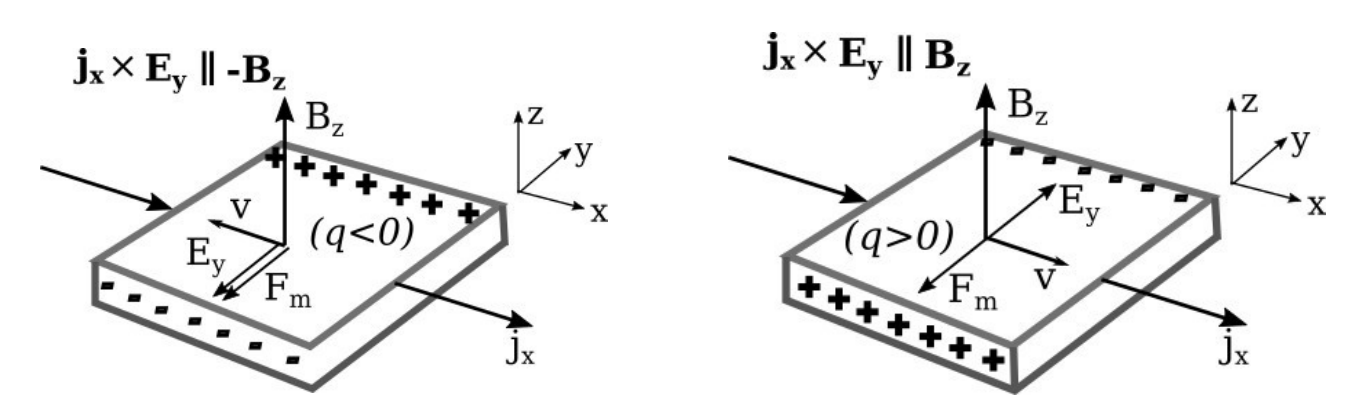
\includegraphics[width=0.8\linewidth]{Cuerpo/Ch_02/Examen_24_6.png}
	      \end{figure}


\end{enumerate}
\vspace*{2em}

\begin{Enunciado}
	\subsubsection{Gap de energía en Ge}
	\begin{minipage}{0.5\linewidth}
		Preguntas
		\begin{enumerate}[label=\alph*)]
			\item Describe el montaje utilizado para la realización de la práctica.
			\item ¿Por qué se utiliza una resistencia de carga (resistencia tampón) en el montaje de la práctica?
			\item Sistemáticamente, se observa una pequeña diferencia entre las curvas conductividad-temperatura a la subida y a la bajada de temperatura. En la gráfica adjunta, ¿qué símbolos corresponden a la bajada y cuáles a la subida?
		\end{enumerate}
	\end{minipage}\hfill
	\begin{minipage}{0.45\linewidth}
		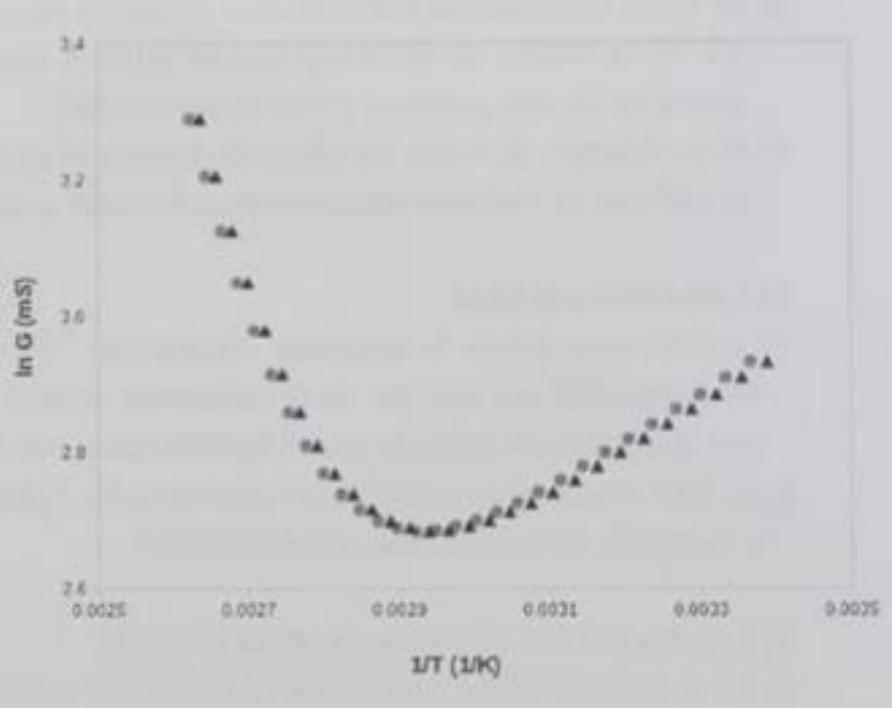
\includegraphics[width=0.9\linewidth]{Cuerpo/Ch_02/Examen_24_7.png}
	\end{minipage}
\end{Enunciado}

Solución:

\begin{enumerate}[label=\alph*)]

	\item El montaje experimental consiste en una placa de Ge-n dopada (20×10×1 mm³), colocada sobre una baquelita portamuestras con calefactor y termómetro incorporados. La corriente que atraviesa el Ge se regula desde el conversor digital-analógico DAC1 del LabJack U6-PRO, y se mantiene en torno a 5 mA mediante una resistencia tampón de 332 Ω colocada en serie.

	      El sistema mide tres voltajes clave:
	      \begin{itemize}
		      \item \( V_{\text{Rt}} \): caída de tensión en la resistencia tampón, que permite calcular la corriente \( I_{\text{Ge}} \)
		      \item \( V_{\text{Ge}} \): caída de tensión en el propio germanio
		      \item \( V_{\text{Pt}} \): voltaje del termómetro de resistencia Pt-100, proporcional a la temperatura de la muestra
	      \end{itemize}

	      La temperatura se regula aplicando corriente al calefactor (resistencia \( R_{\text{cal}} \approx 3.5\ \Omega \)), controlado manualmente. El software registra los datos automáticamente y permite observar en tiempo real la gráfica \( G(T) \), donde \( G = I_{\text{Ge}} / V_{\text{Ge}} \).

	\item La resistencia de carga (o resistencia tampón) de 332 Ω se coloca en serie con la muestra de germanio por dos razones fundamentales:

	      \begin{itemize}
		      \item \textbf{Proteger el germanio}: limita la corriente máxima que puede circular, evitando que se supere el valor recomendado (\( I_{\text{max}} \approx 10\ \text{mA} \)) y previniendo daños térmicos por sobrecorriente.
		      \item \textbf{Medir la corriente indirectamente}: la caída de tensión \( V_{\text{Rt}} \) sobre esta resistencia permite calcular fácilmente la corriente usando la ley de Ohm:
		            \[
			            I_{\text{Ge}} = \frac{V_{\text{Rt}}}{R_{\text{t}}}
		            \]
		            Esto permite obtener la conductancia del germanio sin necesidad de insertar un amperímetro, manteniendo el circuito simple y preciso.
	      \end{itemize}

	\item En el guión se nos indica, que debemos graficar $\ln G$ vs $1/T$, subiendo y bajando para verificar si hay error asociado a la incercia  térmica o al sensor, como podemos ver. La ``incercia  térmica'' basicamente es el proceso por el cual durante la subida de temperatura, el sensor va retrasado respecto la muestra (es decir, se calienta más rápido de lo que el sensor muestra), y durante la bajada, se enfría más lento de lo que el sensor lo indica. Consecuentemente la bajada respecto la curva real está desplazada hacia la derecha y la subia está desplazada hacia la izquierda del valor real: gris circulo subida, negro triángulo bajada. 
\end{enumerate}

\vspace*{2em}

\begin{Enunciado}
	\subsubsection{Efecto Hall en metales}
	Preguntas
	\begin{enumerate}[label=\alph*)]
		\begin{minipage}{0.5\linewidth}
			\item Supongamos que la placa del metal no estuviese a escuadra con el sistema de bobinas, sino que el campo \( \vec{H} \) formase un ángulo de 5° con la normal a la placa. ¿Induciría esto que se obtuviese un valor absoluto del coeficiente Hall \( R_H \) mayor o menor que el real?

		\end{minipage}\hfill\begin{minipage}{0.45\linewidth}
			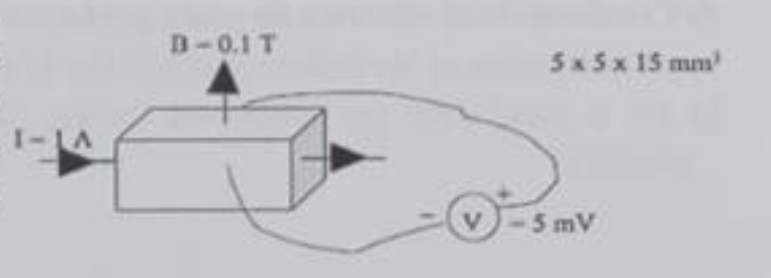
\includegraphics[width=0.9\linewidth]{Cuerpo/Ch_02/Examen_24_8.png}
		\end{minipage}
		\item Una muestra se somete a un campo magnético de \( 0.1\,\text{T} \) y una corriente eléctrica de \( 1\,\text{A} \) como se indica en la figura. A partir del voltaje resultante, determina el signo de los portadores. Suponer que los contactos de voltaje están perfectamente alineados.
	\end{enumerate}
\end{Enunciado}

Solución:

\begin{enumerate}[label=\alph*)]
	\item Como sabemos el coeficiente Hall es el la relación que hay entre el voltaje transversal que se produce por el efecto del campo magnético sobre una corriente, tal que:
	      \[
		      \frac{1}{R_H}\Encal  = \Jn \times \Bn
	      \]
	      tal que, si efectivamente $\Jn = J_x \hnx $ y $\Bn = B_z \hnz$, siempre y cuando midamos  tenemos que:

	      \[
		      R_H = \frac{E_y}{J_x B_z}
	      \]
	      podemos usar el voltaje que aparece entre las terminales $E_y = - V_H d$ donde $d$ es el tamaño de la placa en la dirección. Como podemos ver, esto es deducible a parir de las ecuacioens de Lorentz, en las cuales:

	      \[
		      R_H = \frac{1}{qn}
	      \]
	      Como podemos ver no depende del ángulo de $J_x$ o $B_z$, es una propiedad intrínseca del metal. Si cambiaramos el ángulo tal que $\Jn = J (\cos (\theta) \hnx + \sin (\theta) \hny)$  tendríamos que simplemente mediríamos un $\Encal$ más pequeño, es decir, tendríamos un voltaje más pequeño, no un $R_H$ más pequeño.


	\item Como en el apartado anterior, definimos
	      \[
		      R_H = \frac{E_y}{J_x B_z}
	      \]
	      donde $\hny = \hnx \times \hnz$. Usando las ecuaciones anteriores, tenemos que $E_y = - \Delta V d$, siendo $\Delta V = V_H(d)-V_H(0)$ la difernecia de voltaje entre la placa en $0$ y en $d$. Como podemos ver, en este caso $V_H(0)=0$ y $V_H(d)=-5$ mV, es decir, $R_H$ es positivo y por tanto, por definición esto implica que el signo de los portadores es positivos.


\end{enumerate}

\newpage

\subsection*{\textit{Mayo 2015}}
\addcontentsline{toc}{subsection}{\textit{Mayo 2015}}

\begin{Enunciado}
	\subsection*{Difracción de rayos X}
	\lipsum[1]
\end{Enunciado}

\begin{enumerate}
	\item La ecuación que tenemos que usar es la siguiente:

	      \begin{equation}
		      \sin(\theta)=\frac{\lambda}{2a}\sqrt{h^2+k^2+l^2}
	      \end{equation}

	      No obstante, es necesario particularizarla según el criterio de selección de (h,k,l) para una FCC que es que (h,k,l) deben tener la misma paridad. Teniendo esto en cuenta para las tres primeras ternas que verifican el criterio de selección tenemos:

	      \begin{itemize}
		      \item (1,1,1) $\longrightarrow$ 2$\theta_1$=30.94º
		      \item (2,0,0) $\longrightarrow$ 2$\theta_2$=35.88º
		      \item (2,2,0) $\longrightarrow$ 2$\theta_3$=51.64º
	      \end{itemize}

	\item La no monocromaticidad da lugar a la dispersión de los datos en torno ángulo dado por la $\lambda$ "que más peso tiene".
\end{enumerate}
